\documentclass[12pt,fleqn]{article}
\usepackage{vkCourseML}
\hypersetup{unicode=true}
%\usepackage[a4paper]{geometry}
\usepackage[hyphenbreaks]{breakurl}

\newcommand\xo{\times}
\newcommand\oo{\diamond}

\usepackage[table]{xcolor}  % for clusters examples

\interfootnotelinepenalty=10000

\title{Лекция 17\\Кластеризация}
\author{Е.\,А.\,Соколов, А.\,Гусев, И.\,Садртдинов\\ФКН ВШЭ}
\date{21 февраля 2020 г.}

\begin{document}

\maketitle

Вернемся к одной из задач обучения без учителя --- кластеризации. Пусть у нас есть выборка $ X = \{x_i\}_{i=1}^l, x_i \in \mathbb{X} $, и мы хотим построить алгоритм $ a: \mathbb{X} \rightarrow \{1, ..., K\} $, который  ставил бы в соотвествие объекту номер кластера. Ранее предлагалось использовать номера кластеров как новый признак для обучения с учителем. Сегодня мы рассмотрим модель, которая будет генерировать для нас сколько угодно таких кластерных признаков.

\section{Графовые методы}

\subsection{От выборки к графу}

В курсе МО-1 мы рассматривали несколько алгоритмов кластеризации, а именно:

\begin{itemize}
    \item \textit{K-Means} --- метрический алгоритм, оптимизирующий внутрикластерное расстояние;
    \item \textit{DBSCAN} --- алгоритм, основанный на плотности расположения объектов;
\end{itemize}

Попробуем изобрести немного другой подход. 
Мы можем представить объекты из выборки в виде вершин некоторого неориентированного графа  
$G = (\mathcal{V}, \mathcal{E}),\ \mathcal{V}=X=\{x_1, \dots, x_l\}$.
Рассмотрим несколько вариантов, как в таком представлении можно задать ребра $\mathcal{E}$:

\begin{enumerate}
   \item Граф $G$ может быть полным с ребрами, вес которых определяется по некоторой формуле, например:
   \[
   w_{ij} = \exp\left(-\frac{{\|x_i-x_j\|}^2}{2\sigma^2}\right)\]
   Гиперпараметр $\sigma$ определяет, насколько нам важны далекие объекты.
   \item $G$ можно задать как kNN-граф, то есть объект $x_i$ будет связан с $k$ его ближайшими соседями.
   \item Вершина $x_i$ может быть связана с теми вершинами, расстояние до которых меньше выбранного $\eps$, то есть $\rho(x_i, x_j) < \eps$. Такой граф будет называться $\eps$-графом.
\end{enumerate}

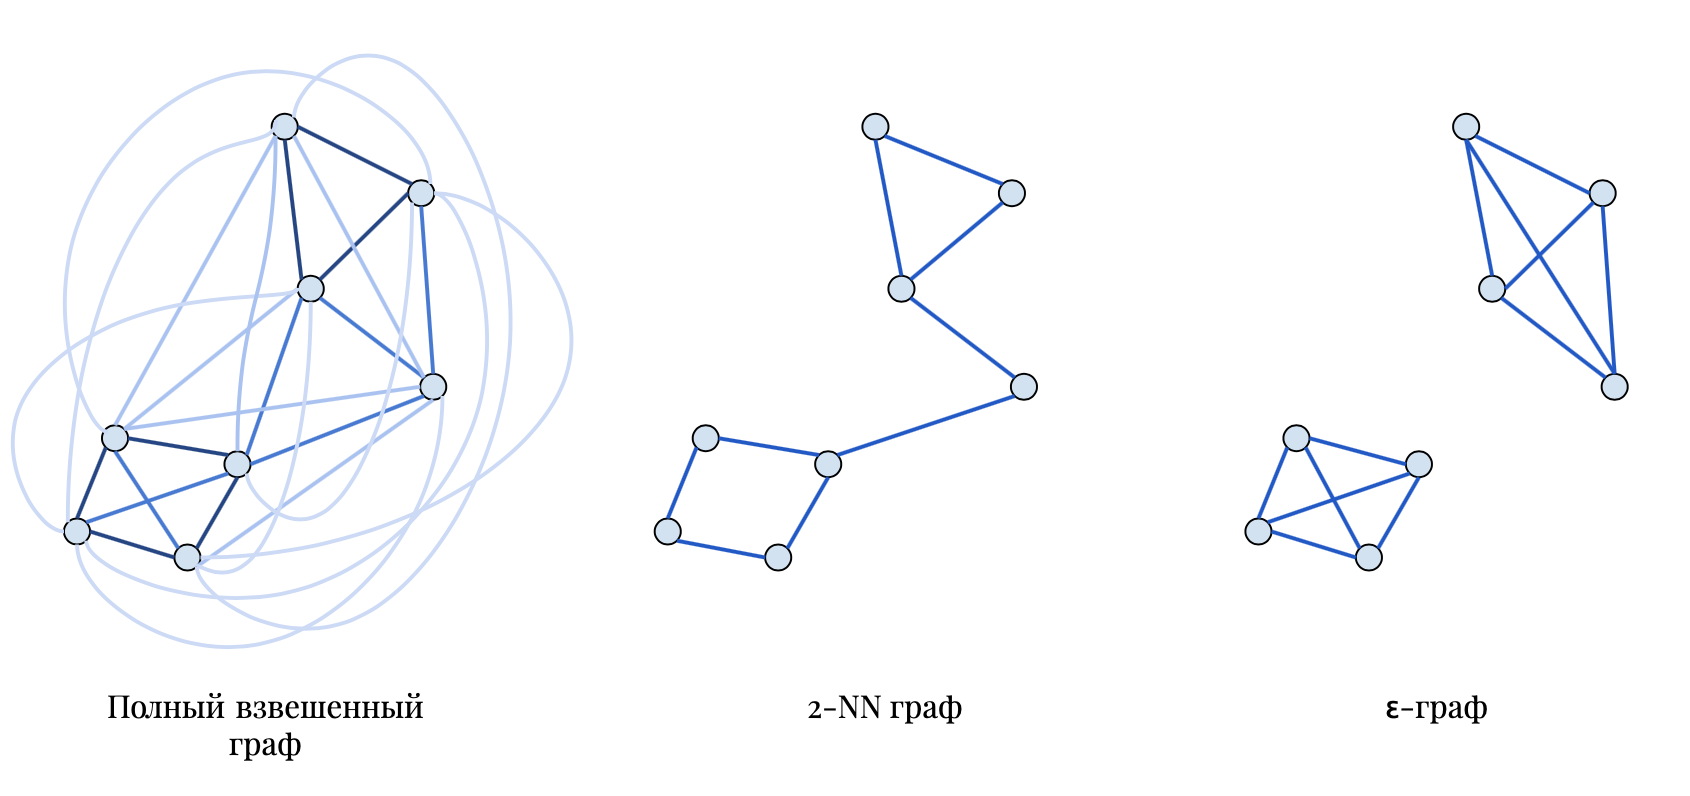
\includegraphics[scale=0.5]{graphs.png}

\subsection{Лапласиан графа}

Обозначим через $W$ матрицу смежности графа $G$. Степени вершин будем считать как $d_i=\sum_{j=1}^{l}w_{ij}$. Пусть $D=\diag(d_1, \dots, d_l)$. Тогда матрица $L=D-W$ будет называться {\it лапласианом} графа $G$. Рассмотрим несколько свойств лапласиана L:

\begin{enumerate}
   \item Пусть $f \in \mathbb R^n$. Тогда имеет место следующая формула:
\[
f^\intercal L f = \frac12 \sum_{i,j=1}^{l}w_{ij}(f_i - f_j)^2
\]

Проверка формулы:
\begin{align*}
f^\intercal L f &= f^\intercal D f - f^\intercal W f = \sum_{i=1}^l d_i f_i^2 - \sum_{i, j = 1}^l w_{ij} f_i f_j = \\
&= \sum_{i=1}^l \left( \sum_{j=1}^l w_{ij} \right) f_i^2 - \sum_{i, j = 1}^l w_{ij} f_i f_j = \sum_{i, j = 1}^l w_{ij} f_i^2 - \sum_{i, j = 1}^l w_{ij} f_i f_j = \\
&= \frac{1}{2} \sum_{i, j = 1}^l w_{ij} f_i^2 + \frac{1}{2} \sum_{i, j = 1}^l w_{ij} f_i^2 - \sum_{i, j = 1}^l w_{ij} f_i f_j = \\
&= \frac{1}{2} \sum_{i, j = 1}^l w_{ij} f_i^2 + \frac{1}{2} \sum_{i, j = 1}^l w_{ij} f_j^2 - \sum_{i, j = 1}^l w_{ij} f_i f_j = \\
&= \frac{1}{2} \sum_{i, j = 1}^l w_{ij}\left(f_i^2 - 2 f_i f_j + f_j^2\right) = \frac{1}{2} \sum_{i, j = 1}^l w_{ij} {\left(f_i - f_j\right)}^2
\end{align*}

   \item $L$ --- симметричная неотрицательно определенная матрица. Симметричность вытекает из неориентированности графа. Свойство неотрицательной определенности легко следует из первого пункта. Действительно, в обсужденных методах постоения графа $w_{ij} \ge 0$, притом $(f_i - f_j)^2 \ge 0$. Следовательно, $f^\intercal L f \ge 0$, что и означает неотрицательную определенность.
   
\end{enumerate}

Однако у лапласиана также есть свойство, которое поможет нам в задаче кластеризации. Сформулируем его в виде теоремы.

\begin{vkTheorem} Пусть $L$ --- лапласиан графа $G$. Тогда выполнены следующие два пункта:
\begin{enumerate}
   \item Собственное значение $\lambda = 0$ матрицы $L$ имеет кратность, равную числу компонент связности $k$.
   \item Пусть $A_1, \dots, A_k$ --- компоненты связности графа $G$. Тогда векторы $f_1,\dots, f_k$, определяемые по формуле
   $f_i = \left([x_j\in A_i]\right)_{j=1}^{l}$, будут являться собственными векторами для $\lambda = 0$.
\end{enumerate}
\end{vkTheorem}
\begin{vkProof}
Сперва рассмотрим случай $k=1$. Поймем, почему $\lambda=0$ вообще является собственным значением матрицы $L$. Для этого рассмотрим вектор $f=(1,\dots,1)$:

\begin{gather*}
L f = D f - W f =
\begin{pmatrix}
d_1&0&\cdots &0\\ 
0&d_2&\cdots &0\\
\vdots &\vdots &\ddots &\vdots \\
0&0&\cdots & d_l
\end{pmatrix}
\begin{pmatrix}
1 \\
\vdots \\
1
\end{pmatrix} - 
\begin{pmatrix}
w_{11}&w_{12}&\cdots &w_{1l}\\ 
w_{21}&w_{22}&\cdots &w_{2l}\\
\vdots &\vdots &\ddots &\vdots \\
w_{l1}&w_{l2}&\cdots & w_{ll}
\end{pmatrix}
\begin{pmatrix}
1 \\
\vdots \\
1
\end{pmatrix} = \\
= \begin{pmatrix}
d_1 \\
\vdots \\
d_l
\end{pmatrix} -
\begin{pmatrix}
w_{11} + \dots + w_{1l} \\
\vdots \\
w_{l1} + \dots + w_{ll}
\end{pmatrix} = 0
\end{gather*}

Теперь предположим, что существует собственный вектор $f'\in \mathbb R^n:\ \exists p\ne q \rightarrow f'_p \ne f'_q$, то есть неконстантный вектор, соответствующий $\lambda =0$. Тогда $Lf'=0 \Rightarrow f'^\intercal L f'=0$. Но рассматриваемый граф является связным. Значит существует путь 
$p = i_0 \rightarrow i_1 \rightarrow \dots \rightarrow i_{n-1} \rightarrow i_n = q$. Поскольку вершины $i_r$ и $i_{r+1}$ соединены ребром, то $w_{i_r i_{r+1}} > 0 $, а значит, $f'_{i_r} = f'_{i_{r+1}}$ (иначе получим $ f'^\intercal L f' > 0$). Отсюда $f'_p=f'_{i_1} = \dots = f'_{i_{n-1}}=f'_q$ - константный вектор. Получили противоречие $\Rightarrow$ $f'$ не является собственным вектором для $\lambda=0$. Значит, мы доказали оба пункта для $k=1$.

Теперь пусть $k>1$. Можно упорядочить вершины так, чтобы лапласиан $L$ стал блочно-диагональной матрицей:

\[
L =
\begin{pmatrix}
L_1&0&\cdots &0\\ 
0&L_2&\cdots &0\\
\vdots &\vdots &\ddots &\vdots \\
0&0&\cdots & L_k
\end{pmatrix}
\]

Блоки $L_1, \dots, L_k$ будут являться лапласианами компонент связности графа $G\ \Rightarrow\ \lambda=0$ имеет кратность $k$, а собственные векторы $f_1, \dots, f_k$ задаются по формуле 
\[
f_i = \left([x_j\in A_i]\right)_{j=1}^{l}
\]
\end{vkProof}

\begin{vkHypothesis}
Пусть есть похожие объекты $x_j$ и $x_k$, то есть расстояние между ними невелико.
Тогда у собственных векторов $f_i$, соответствующих маленьким собственным значениям, выполнено $f_{ij} \approx f_{ik}$. 
\end{vkHypothesis}

Эта гипотеза имеет лишь эмпирическое доказательство. Однако алгоритм, построенный на этой гипотезе, позволяет достигать успеха в задаче кластеризации. Данный алгоритм называется {\it спектральной кластеризацией}.

\subsection{Спектральная кластеризация}

{\bf Алгоритм спектральной кластеризации:}
\null\hfill {\it Сложность шага}
\begin{enumerate}
    \item Строим по объектам граф $G$ и лапласиан $L = D - W$.
    \null\hfill $\mathcal{O}(l^2)$
    \item Находим нормированные собственные векторы $u_1, \dots, u_m$ матрицы $L$, \par соответствующие $m$ наименьшим собственным значениям.  \null\hfill $\mathcal{O}(l^3)$
    \item Составляем матрицу $U \in \mathbb R^{l \times m}$:
    $U = (u_1 | \dots | u_m)$.
    \null\hfill$\mathcal{O}(lm)$
    \item Обучаем на этой матрице алгоритм K-Means c $k$ кластерами.
   \null\hfill$\mathcal{O}(l^{mk+1})$
\end{enumerate}

Если мы верим в нашу гипотезу, то для похожих объектов соответствующие координаты векторов $u_1, \dots, u_m$ будут близки. Матрица $U$ имеет размерность $l\times m$, поэтому можно посмотреть на нее, как на матрицу объекты-признаки. При этом новыми признаками будут как раз собственные вектора $u_1, \dots, u_m$. В описанном выше алгоритме предлагается обучать на них K-Means, но никто не запрещает использовать эти признаки для других задач.

Как видно, алгоритм обладает высокой вычислительной сложностью. Но утверждается, что он позволяет достигать впечатлящих результатов в задаче кластеризации. Однако как оценить, насколько хорошо алгоритм справляется с задачей классификации? Этому вопросу посвящен остаток лекции.

\section{Оценка качества кластеризации}

\subsection{Метрика на разметке}

Пусть существует разметка $(y_1, \dots, y_l)$, не участвующая при обучении. Мы не использовали эту разметку в качестве дополнительного признака, так как нам не хочется мотивировать модель данным признаком. Тогда предлагается ввести оценку качества алгоритма кластеризации при помощи этой разметки, саму же разметку тогда называют {\it gold standard}. Введем несколько требований к внешней метрике качества $Q$:

\begin{enumerate}
    \item \textit{Гомогенность}. Базовое свойство разделения разных объектов в разные кластеры:
\[Q
  \left(\begin{array}{ccc}
     &  \cellcolor{red!10} \oo &  \cellcolor{red!10}\oo \\
    \cellcolor{red!10} \xo  &  \cellcolor{red!10} &  \cellcolor{red!10} \oo \\
    \cellcolor{red!10} \xo  & \cellcolor{red!10} \xo  & \\
  \end{array}\right)
  <
  Q
  \left(\begin{array}{ccc}
     &  \cellcolor{green!10} \oo &  \cellcolor{green!10}\oo \\
    \cellcolor{red!10} \xo  &   &  \cellcolor{green!10} \oo \\
    \cellcolor{red!10} \xo  & \cellcolor{red!10} \xo  & \\
  \end{array}\right)
\]
    \item \textit{Полнота}. Один кластер не должен дробиться на несколько маленьких:
\[  Q
  \left(\begin{array}{ccc}
     &  \cellcolor{green!10} \xo &  \cellcolor{green!10}\xo \\
    \cellcolor{red!10} \xo  &   &  \cellcolor{green!10} \xo \\
    \cellcolor{red!10} \xo  & \cellcolor{red!10} \xo  & \\
  \end{array}\right)
<
Q
  \left(\begin{array}{ccc}
     &  \cellcolor{red!10} \xo &  \cellcolor{red!10}\xo \\
    \cellcolor{red!10} \xo  &  \cellcolor{red!10} &  \cellcolor{red!10} \xo \\
    \cellcolor{red!10} \xo  & \cellcolor{red!10} \xo  & \\
  \end{array}\right)
\]
    \item \textit{Rag-bag}. Весь мусор должен быть в одном "мусорном"  кластере, чтобы остальные кластеры были "чистыми":
    \[  Q
  \left(\begin{array}{cccc}
    \cellcolor{red!10} \xo & \cellcolor{red!10} \xo &  \cellcolor{green!10} \bullet & \cellcolor{green!10} \circ \\    
    \cellcolor{red!10} \xo & \cellcolor{red!10} \xo &  \cellcolor{green!10} \triangleright & \cellcolor{green!10} \star \\    
    \cellcolor{red!10} \xo & \cellcolor{red!10} \ast &  \cellcolor{green!10}\odot & \cellcolor{green!10} \Box \\
  \end{array}\right)
  <
  Q
  \left(\begin{array}{cccc}
    \cellcolor{red!10} \xo & \cellcolor{red!10} \xo &  \cellcolor{green!10} \bullet & \cellcolor{green!10} \circ \\    
    \cellcolor{red!10} \xo & \cellcolor{red!10} \xo &  \cellcolor{green!10} \triangleright & \cellcolor{green!10} \star \\    
    \cellcolor{red!10} \xo & \cellcolor{green!10} \ast &  \cellcolor{green!10}\odot & \cellcolor{green!10} \Box \\
  \end{array}\right)
  \]
  \item {\it Cluster size vs. quantity.} Лучше испортить один кластер с целью улучшить качество множества других:
  \[
  Q
  \left(\begin{array}{cccc}
    \cellcolor{red!10} \xo &  &  \cellcolor{green!10} \circ & \cellcolor{cyan!10} \circ \\    
    \cellcolor{red!10} \xo &  &  \cellcolor{violet!10} \star & \cellcolor{black!10} \star \\    
    \cellcolor{red!10} \xo &  &  \cellcolor{brown!10}\triangleright & \cellcolor{gray!10} \triangleright \\
    \cellcolor{red!10} \xo &  &  \cellcolor{yellow!10}\odot & \cellcolor{orange!10} \odot \\
  \end{array}\right)
  <
  Q
  \left(\begin{array}{cccc}
    \cellcolor{red!10} \xo &  &  \cellcolor{green!10} \circ & \cellcolor{green!10} \circ \\    
    \cellcolor{red!10} \xo &  &  \cellcolor{violet!10} \star & \cellcolor{violet!10} \star \\    
    \cellcolor{red!10} \xo &  &  \cellcolor{brown!10}\triangleright & \cellcolor{brown!10} \triangleright \\
    \cellcolor{blue!10} \xo &  &  \cellcolor{yellow!10}\odot & \cellcolor{yellow!10} \odot \\
  \end{array}\right)
  \]
\end{enumerate}
  
\subsection{BCubed}

Единственной известной на данный момент метрикой, обладающей всеми четыремя названными свойствами является BCubed. Она считается следующим способом. Пусть $L(x)$ --- gold standard, $C(x)$ --- номер кластера, выдаваемый рассматриваемым алгоритмом. Тогда рассмотрим несколько величин:

\[
\mathsf{Correctness}(x, x') = 
\begin{cases} 
1 &,\ C(x) = C(x') \wedge L(x) = L(x') \\ 
0 &,\ otherwise
\end{cases}
\]
\[
\mathsf{Precision\mbox{-}BCubed} = \mathsf{Avg}_x \left[\mathsf{Avg}_{x':C(x)=C(x')}\mathsf{Correctness}(x, x')\right]
\]
\[
\mathsf{Recall\mbox{-}BCubed} = \mathsf{Avg}_x \left[\mathsf{Avg}_{x':L(x)=L(x')}\mathsf{Correctness}(x, x')\right]
\]

Тогда $\mathsf F$-мера от определенных точности и полноты будет удволетворять всем нужным нам требованиям.

\begin{vkExample}
\[
\begin{array}{ccc}
     &  \cellcolor{green!10} \xo &  \cellcolor{green!10}\xo \\
    \cellcolor{red!10} \xo  &   &  \cellcolor{green!10} \xo \\
    \cellcolor{red!10} \xo  & \cellcolor{red!10} \xo  & \\
\end{array} \\
\mathsf{Precision\mbox{-}BCubed} = 1, \\
\mathsf{Recall\mbox{-}BCubed} = \frac12, \\
\mathsf{BCubed} = \frac{1 \cdot \frac{1}{2}}{1 + \frac{1}{2}} = \frac{1}{3}
\]
\end{vkExample}

\end{document}
